\documentclass[12pt]{extarticle}
\usepackage[utf8]{inputenc}
\usepackage{amsmath}
\usepackage{graphicx}

\title{MATH 377: Model Fitting Assignment}
\author{Connor Gephart}
\date{22 October 2019}

\begin{document}

\maketitle
\section{Introduction}
This project is an introduction to model fitting for several sets of example data. The goal was to find a model that best fit the given data, and to draw up some graphs to defend that it is the best. There were three data sets given: Wire Stress, Pines, and Planets. Each set is detailed below. 

\section{Wire Stress}
\subsection{Scatter Plot}
The Wire Stress data is the elongation, in $10^{-5}$ inches per inch, of a certain wire based upon how much stress, in pounds per inch squared, is applied to it. The data is shown in the following scatter plot, with the linear trend line applied. It can be seen that this function is quite appropriate for the data, with an $R^2$ value of $0.9989$. A polynomial trend line could also be applied, but this runs the risk of overfitting the model for this specific set of experimental data. 
\newpage
\begin{figure}[ht!]
  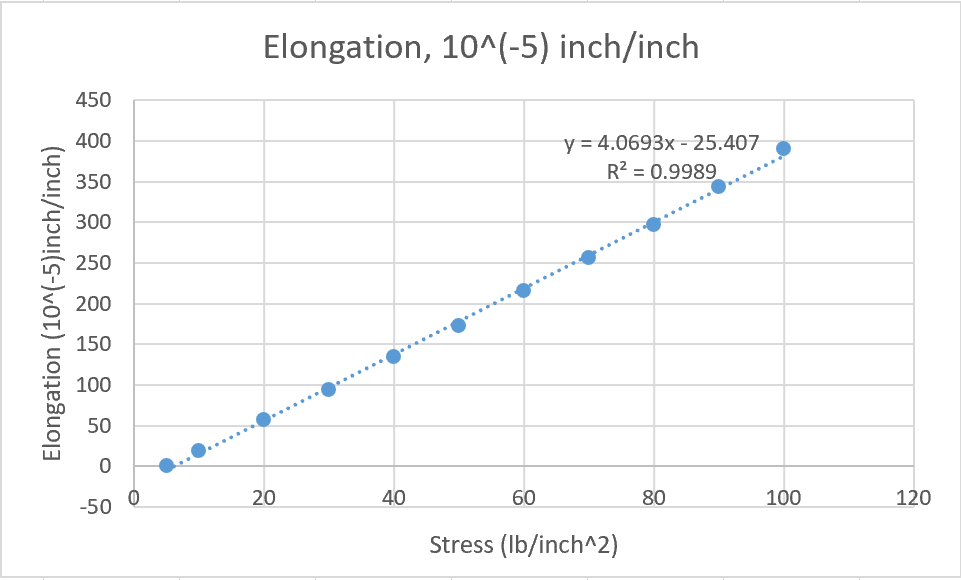
\includegraphics[width=\linewidth]{ElongationScatter.PNG}
  \caption{Wire stress v. elongation scatter plot}
\end{figure}
\newpage
\subsection{Residuals}
However, it is often best to try to simplify the models to make them easier to deal with. In this case, the equation can be rounded to the following: $y = 4.07x - 25.4$. This can then be compared by plotting the residuals between this model and the actual data, shown below. The largest difference is off by approximately 2\% so this model is a decent representation of the data, and would be good to use as a predictor.
\begin{figure}[ht!]
  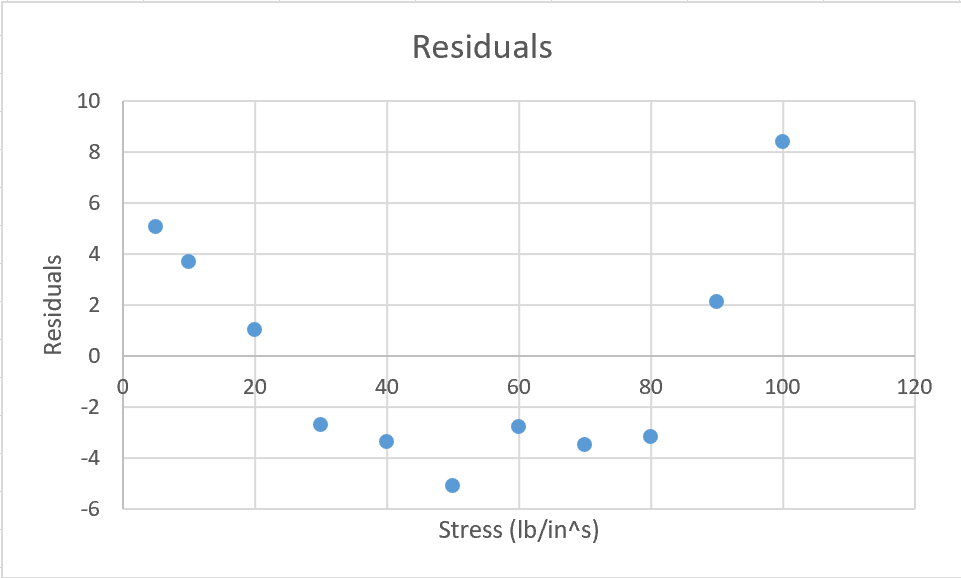
\includegraphics[width=\linewidth]{ElongationResiduals.PNG}
  \caption{wire stress residuals plot}
\end{figure}
\newpage
\section{Pines}
\subsection{Scatter Plot}
The next data set compares the diameter, in inches, of a pine tree to the volume, in board feet per 10, of wood. The data has a power trend line applied below, with an $R^2$ value of $0.9858$. 
\begin{figure}[ht!]
  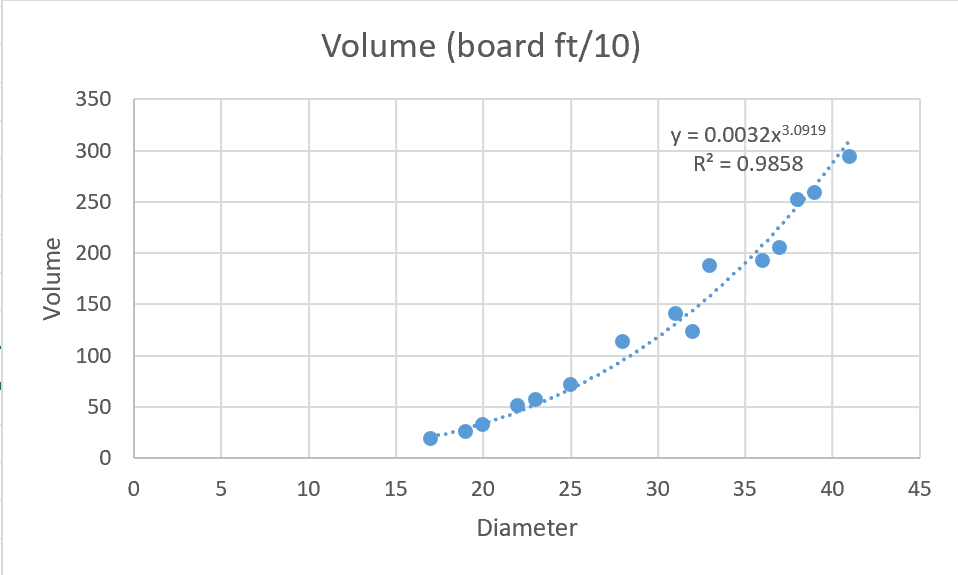
\includegraphics[width=\linewidth]{PineScatter.PNG}
  \caption{Pine diameter v. volume scatter plot}
\end{figure}
\newpage
\subsection{Residuals}
The practical application of this model would be for lumber workers who wish to know if a tree should be cut down based on its diameter. The equation given in the above graph is $y = 0.0032x^{3.0919}$, which is not the easiest formula to remember or use. The moderately simplified equation $y = 0.0032x^{3.1}$ is used to generate the residual plot below. The coefficient of $0.0032$ can be understood as applying the formula to large quantities of wood. This model is slightly worse for fit than with the wire stress above, but it still does a good job and is only 8\% incorrect at most. 
\begin{figure}[ht!]
  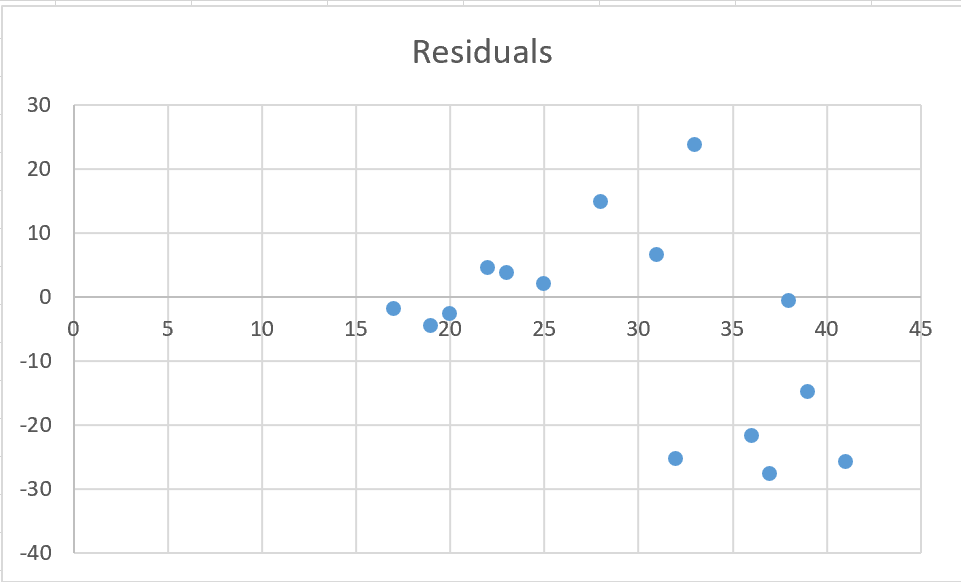
\includegraphics[width=\linewidth]{PineResiduals.PNG}
  \caption{Pine residuals plot}
\end{figure}

\section{Planets}
The goal of this set of data is to derive one of Kepler's Laws about the length of a planet's period, in days, and the minimum distance from the sun, in millions of kilometers. Similar to the pines data, a power trend line is applied to the data, but this time with $R^2 = 1$. However, comparing the equation of this line, $y=2.9403x^{0.6659}$ to the actual equation, $y=3x^{\frac{2}{3}}$ shows this to be an example of overfitting. The original scatter plot of the data, and then the scatter plot of the residuals using the actual equation are shown below. The residuals show a largest difference of 3\% when using the model to approximate actual data.  
\begin{figure}[ht!]
  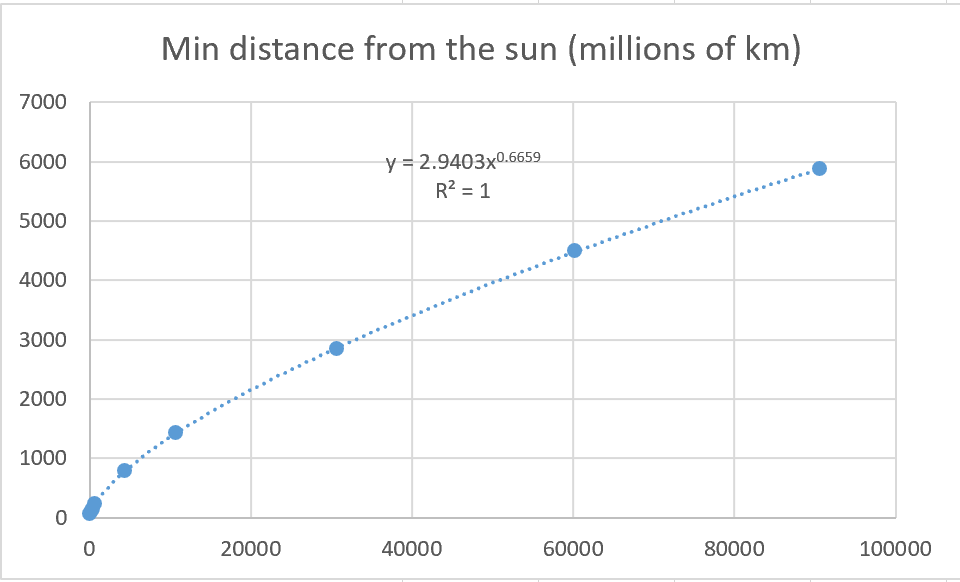
\includegraphics[width=\linewidth]{PlanetsScatter.PNG}
  \caption{Planets period v. minimum distance from sun scatter plot}
\end{figure}
\begin{figure}[ht!]
  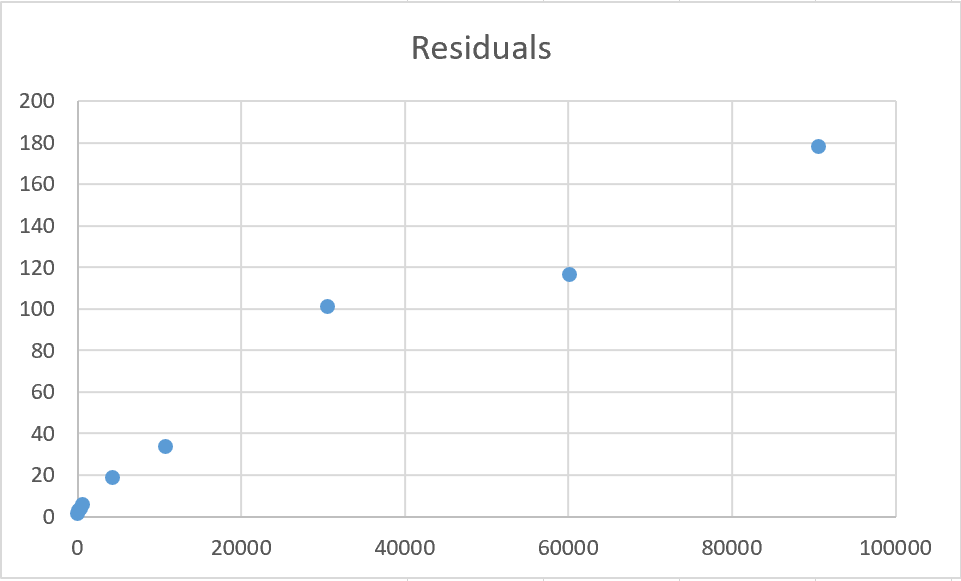
\includegraphics[width=\linewidth]{PlanetsResiduals.PNG}
  \caption{Planets residuals plot}
\end{figure}

\end{document}